\documentclass[11pt]{article}
\usepackage[review]{acl}
% The NAACL 2027 demo track is single-blind. Keep review line/page numbers,
% while identifying the author; the official style file is unmodified.
\makeatletter
\acl@anonymizefalse
\makeatother
\usepackage{times}
\usepackage{latexsym}
\usepackage[T1]{fontenc}
\usepackage[utf8]{inputenc}
\usepackage{microtype}
\usepackage{inconsolata}
\usepackage{graphicx}
\usepackage{booktabs}
\usepackage{amsmath}
\usepackage{tikz}
\usetikzlibrary{arrows.meta,positioning}

\newcommand{\system}{Mini Jev}
\newcommand{\CodeURL}{\href{https://github.com/UpHash-Network/mini-jev/tree/research/naacl2027-demo}{github.com/UpHash-Network/mini-jev}}
% Public recording URL is verified against the published branch before delivery.
\newcommand{\DemoVideo}{\href{https://raw.githubusercontent.com/UpHash-Network/mini-jev/refs/heads/research/eacl2027-demo/paper/eacl2027/Mini_Jev_Demonstration.mp4}{approximately 145-second captioned live recording}}

\title{Mini Jev: An Inspectable Local Interface for Typed Decisions\newline from Frozen Language Models}
\author{Yuki Oshio \\
  UPHASH Inc. \\
  \texttt{oshio@uphash.net}}

\begin{document}
\maketitle

\begin{abstract}
Many language-model applications need a small typed decision rather than free-form text. \system{} is an open-source local interface that maps a state and explicit criteria to a categorical choice, a true-candidate probability, or an expected ordinal stage. It uses candidate next-token logits from a frozen language model, with no trained decision head. A browser demonstration exposes typed values, candidate distributions, probability semantics, and request/response JSON. A 4,050-request matched comparison finds identical direct-readout and native one-token outputs in all 1,350 pairs, without an established latency advantage. Two subsequent studies across three checkpoints use 7,600 and 14,400 requests to examine presentation sensitivity and probability averaging. Reduced sensitivity can coexist with incorrect or nearly constant predictions, while averaging costs multiple model calls. The contribution is a runnable demonstration and auditable system evaluation, with explicit distinctions among type validity, candidate concentration, task quality, and computation cost.
\end{abstract}

\section{Introduction}
A workflow may need a route, an urgency score, or a stage on an explicit rubric. Returning a paragraph and then recovering that value creates an interface problem: the application must validate a result whose useful content is small. A typed interface makes the contract explicit, but a valid type alone says nothing about whether the decision is right. Similarly, a model can assign almost all candidate probability to an incorrect answer.

\system{} demonstrates this distinction through a local browser interface and an HTTP/Python API. Users edit a shared state and three questions, run the model, and inspect the resulting values alongside candidate distributions. The interface is inspired by TypeSafe's Jev \citep{typesafe2026jev,typesafeapi}; this independent implementation makes no claim to reproduce that system's architecture, training, calibration, compatibility, or performance.

The intended users are developers and researchers inspecting small typed decisions from local frozen models before integrating them into a workflow. The mechanism is conventional: a frozen model scores explicit single-token candidates, a restricted softmax produces a distribution, and ordinary code constructs the typed response. Verbalizers, logit-based candidate selection, and candidate-scoring APIs are established \citep{schick2021pet,ma2025inferring,lmqlscoring}. Our contribution is a runnable interface for inspecting typed readouts and their probability semantics, together with an auditable evaluation of quality, presentation sensitivity, and computation cost. We do not claim a new scoring method or the first model-inspection interface.

Schema validity, regression checks, task quality, and paired timing answer different questions. Our matched study finds no material latency advantage over native one-token selection. Source, installation, data documentation, and evaluation artifacts: \CodeURL. Video: \DemoVideo.

\section{System and Typed Contract}
\label{sec:system}
\subsection{From a state to typed values}
A request contains a shared \texttt{state} and named questions. Each question supplies a type, natural-language instructions, and candidate criteria. The service returns a semantic label, a candidate distribution, and a type-specific value:
\begin{itemize}
  \item \textbf{Choice} returns the key of the most likely candidate. Keys are canonically sorted before prompting.
  \item \textbf{Noul} exposes the probability of the \texttt{true} candidate in a two-candidate false/true decision.
  \item \textbf{Score} returns the expected zero-based stage of an ordered rubric; the most likely stage is also available as the label.
\end{itemize}
The distinction between Score's expectation and its hard label matters. An expectation of 1.6 on stages 0--3 is a probability-weighted position, not an additional model-generated stage or a calibrated utility. Its interpretation assumes equally spaced stage indices; users must decide whether that fits their rubric.

Let $z_i$ denote the next-token logit for candidate $i\in\{0,\ldots,K-1\}$, with $K$ candidates and temperature $T>0$. The service computes
\begin{equation}
\begin{aligned}
 p_i &= \frac{\exp(z_i/T)}{\sum_{j=0}^{K-1}\exp(z_j/T)},\\
 s &= \sum_{i=0}^{K-1} i p_i.
\end{aligned}
\end{equation}
These are probabilities conditional on the selected candidate set. They are neither probabilities over all valid textual answers nor guarantees that the criteria are exhaustive. Changing the criteria changes the question as well as the normalization. The optional scalar temperature preserves the maximum-logit label, but can change Noul and Score values.

The interface also displays entropy concentration,
\begin{equation}
\begin{aligned}
 c &= 1 - H(p)/\log K,\\
 H(p) &= -\sum_i p_i\log p_i.
\end{aligned}
\end{equation}
A concentrated distribution has $c$ near one. The display identifies this quantity as concentration rather than estimated accuracy. The response includes probability-semantics and calibration metadata, so downstream applications can retain the same distinction.

\subsection{Local execution}
The released inference configuration uses Qwen3.6-35B-A3B in Q4\_K\_M GGUF form \citep{qwen36,qwen36gguf}, through a source-built \texttt{llama.cpp} helper \citep{llamacpp}. The model and its output projection remain frozen; there is no trained decision head. The helper performs the full vocabulary projection and then gathers candidate logits. It does not implement a selected-row projection optimization.

The prompt repeats the task twice, following the use of repetition for non-reasoning inference \citep{leviathan2025repetition}. Choice and Noul use letter labels; Score with at most ten stages uses digits after a prefilled answer-object prefix. Larger Score rubrics use letters. The implementation checks that every candidate is a distinct single token at the actual prefix boundary. The API accepts 2--26 candidates; quality evaluation covers 2--8, while larger candidate sets have functional coverage only.

A multi-question request executes its questions sequentially. Model state is cleared between questions: they share the supplied state text, but not a cached prefill. Complete inputs exceeding 2,048 tokens are rejected rather than silently truncated. Schema validation and deterministic response construction prevent free-form output from crossing the API boundary; these software properties do not prevent semantic errors.

\begin{figure}[t]
\centering
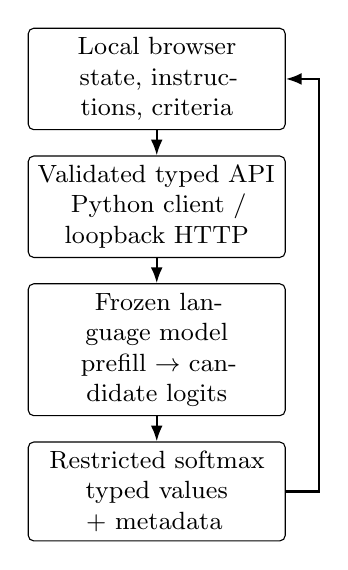
\begin{tikzpicture}[
  box/.style={draw,rounded corners=2pt,align=center,text width=3.03cm,minimum height=.72cm,font=\small},
  arr/.style={-{Latex[length=2mm]},thick},node distance=.32cm]
\node[box] (ui) {Local browser\\state, instructions, criteria};
\node[box,below=of ui] (api) {Validated typed API\\Python client / loopback HTTP};
\node[box,below=of api] (lm) {Frozen language model\\prefill $\rightarrow$ candidate logits};
\node[box,below=of lm] (readout) {Restricted softmax\\typed values + metadata};
\draw[arr] (ui)--(api);
\draw[arr] (api)--(lm);
\draw[arr] (lm)--(readout);
\draw[arr] (readout.east)--++(.42,0)|-(ui.east);
\end{tikzpicture}
\caption{The live demonstration uses the released typed API. It displays model-derived candidate distributions and typed values; no generated explanation or simulated prediction is inserted.}
\label{fig:architecture}
\end{figure}

\subsection{Relationship to one-token decoding}
Restricted softmax readout has the same mathematical candidate distribution as a sampler that masks all non-candidates, provided the model prefix, logits, candidate IDs, temperature, and other processors match. Greedy labels then agree unless tie-breaking differs; stochastic sampling agrees in distribution, not necessarily in realized samples. This is an equivalence under specified conditions, not a new inference theorem or learning method.

In particular, selecting a first token after prefill need not require another model forward pass. Avoiding a generated token therefore does not itself establish a speedup. The matched study in Section~\ref{sec:evidence} tests this point using an actual native one-token sampler, rather than comparing direct readout only with a long textual answer.

\section{Demonstration and Access}
\label{sec:demo}
The browser runs locally and connects through a small Python bridge to the existing model API. It requires no cloud inference service. A user starts with a shared state and three editable questions: routing through Choice, urgency through Noul, and priority through Score. The question instructions and criteria are visible, making the decision contract available for inspection before inference.

The user defines the state and criteria and selects \emph{Run decisions}. Candidate probabilities distinguish a hard label from its distribution; Score's expected and most likely stages can differ. Rerunning after edits explores behavior, but changes the input and is not a controlled accuracy experiment.

The page also displays entropy concentration, elapsed time, and copyable request/response JSON. The bars show relative candidate mass, the JSON exposes the contract, and elapsed time describes the live request; none is a reference answer. Editing marks prior results stale. There is no replay mode: an unavailable model API produces an error, not a canned prediction.

% The figure is a captured live demonstration, not a synthetic mockup.
\IfFileExists{figures/demo-presentation.png}{%
\begin{figure*}[t]
\centering
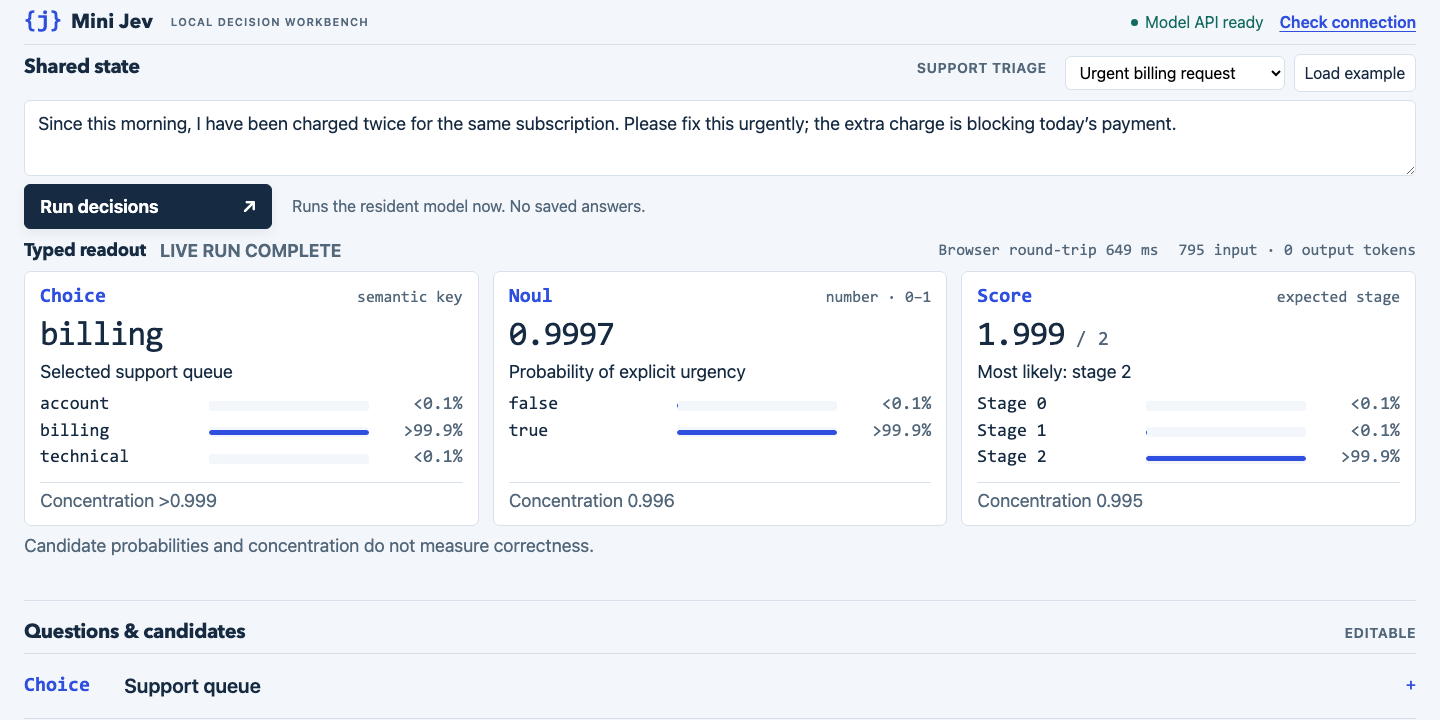
\includegraphics[width=\textwidth]{figures/demo-presentation.png}
\caption{Live browser demonstration in presentation view: an editable state, all three typed outputs, and their candidate distributions. The question editors continue below the displayed results. This English example illustrates the interface; it is not an evaluation item or evidence of English task quality.}
\label{fig:demo}
\end{figure*}}{}

Installation begins with the repository's native build script and pinned model downloader. Users build the helper with \texttt{build\_native.sh}, download the model with \texttt{fetch\_native\_model.py}, and start the API with \texttt{./run.sh --without-calibration}. Starting \texttt{python3 -m demo.server --port 8766} then opens access at \url{http://127.0.0.1:8766/}. The repository supplies complete commands and a Python client example. Fresh builds start at $T=1$; historical calibration artifacts are bound to their recorded runtime and should not silently transfer to a different build.

The tested environment is an Apple M5 Pro with 64\,GB unified memory and macOS 26.4, using Metal and Accelerate. The model file is approximately 20.4\,GB, in addition to runtime memory. This is a local workstation demonstration, not a claim of lightweight deployment or a demonstrated minimum-memory requirement. Source is distributed; model weights and compiled native binaries are not bundled.

\section{Evidence Behind the Demonstration}
\label{sec:evidence}
\subsection{Evaluation panels and provenance}
Table~\ref{tab:sets} separates the evidence sources. Repeated requests are not additional quality examples, and the external tasks do not share one accuracy metric.

\begin{table}[t]
\centering
\small
\setlength{\tabcolsep}{3pt}
\begin{tabular}{@{}p{1.72cm}p{1.44cm}p{4.08cm}@{}}
\toprule
Evidence & Size & Interpretation \\
\midrule
Local regression & 2,400 items & Self-authored Japanese; 800 per type \\
Expanded external & 600 items & JCoLA, JSTS, JCQA; 200 each \\
Matched runtime & 4,050 requests & 150 local $\times$ 5 repetitions, plus 600 external; 3 modes \\
Presentation study & 7,600 requests & Same 600 external items; 3 checkpoints \\
Cyclic averaging & 14,400 requests & 600 additional external items; 3 checkpoints \\
\bottomrule
\end{tabular}
\caption{Evaluation accounting. The last two studies use 1,200 unique source items in total. Measured counts exclude synthetic checks and warm-ups. JCQA abbreviates JCommonsenseQA.}
\label{tab:sets}
\end{table}

The historical local suite contains 2,220 generated items from 45 template families and 180 individually AI-authored items; its legacy \texttt{manual} field does not mean human annotation. Authoring used earlier development errors, so it is regression material rather than a blind external test. All 2,400 outputs were valid, but 162 top labels were wrong: structural validity does not establish correctness. Historical temperature fitting also did not improve all calibration and score-error metrics.

The expanded sample has 200 public-development examples each from JCoLA \citep{someya2024jcola}, JSTS, and JCommonsenseQA \citep{kurihara2022jglue}. Hash selection and rubrics were frozen before inference, without independent preregistration. Six JSTS rows share text or image provenance with an earlier 300-item JNLI pilot. Public development data may have appeared in model training; these are not independent hidden-test evaluations.

\subsection{Matched runtime and parity}
All three conditions used one resident model and a common research HTTP response containing a type and semantic label. Direct readout and native one-token greedy selection used identical complete prompts and candidates. The JSON condition actually generated a grammar-constrained object, with a serialization-specific prompt. Its timing comparison therefore includes prompt and prefill differences as well as multi-token generation; it does not isolate sampler overhead.

The schedule contained $(150\times5+600)\times3=4{,}050$ measured requests, plus 21 synthetic warm-ups. All completed with valid responses and no recorded HTTP failures. Mode order was randomized within each item/repetition. Timing covered serialization through loopback HTTP parsing, including native audit transfer but excluding trace-file writes. These are research-harness timings, not browser rendering times.

Direct and one-token conditions matched prompts, token sequences, candidate IDs, logits, and labels in all 1,350 paired observations. Maximum observed candidate-logit difference was zero; there were no maximum-logit ties. The primary latency statistic is the median across 150 local items of the within-item difference between five-repetition mean latencies. It is not a difference between marginal medians.

\begin{table}[t]
\centering
\small
\setlength{\tabcolsep}{3pt}
\begin{tabular}{@{}lrr@{}}
\toprule
Comparator $-$ direct & Difference & 95\% interval \\
\midrule
One token & $+0.0898$ & $[-0.7483,\;0.8449]$ \\
JSON & $+160.2958$ & $[138.1189,\;177.0587]$ \\
\bottomrule
\end{tabular}
\caption{Primary paired HTTP latency differences in milliseconds. Intervals resample observed local family/tag clusters; JSON uses a different serialization prompt.}
\label{tab:latency}
\end{table}

Table~\ref{tab:latency} gives 10,000-replicate whole-family/tag percentile intervals. They describe sensitivity to the observed cluster composition, conditional on this model, machine, selected items, and session. They do not estimate between-machine or independent-session variability. The one-token interval crosses zero: this run provides no evidence of a material direct-readout latency advantage. JSON was slower under its different serialization requirements, with task-dependent quality changes.

\subsection{External task-specific results}
Direct readout and one-token selection have identical external labels. JCoLA reached 86.0\% accuracy and MCC 0.5708; JSON reached 82.0\% and MCC 0.5160. The selected sample contains 158 acceptable sentences, so an always-acceptable rule already achieves 79.0\% accuracy and has undefined MCC. Reporting only accuracy would obscure this imbalance.

JCommonsenseQA accuracy was 95.0\% for direct/one-token and 95.5\% for JSON, a difference of one example. JSTS retains its continuous reference scores in $[0,5]$: direct expected-stage MAE at $T=1$ was 0.5065. JSON has no comparable probability vector, so we do not assign it an expected-stage metric. The separate hard-stage comparison gives MAE 0.5480 for direct/one-token and 0.5650 for JSON. We do not round the gold scores into invented classes or pool these tasks into one accuracy.

\subsection{Presentation sensitivity and averaging}
Two subsequent studies add Qwen2.5-0.5B-Instruct and Qwen2.5-1.5B-Instruct to the native 35B checkpoint. The first uses 7,600 requests on the same 600 external items. All 1,800 exact-input repeat pairs have identical logits and probabilities, yet display reversal changes native JCQA labels on 11/200 items. Conversely, the 1.5B checkpoint has zero JCoLA flips while always predicting acceptable: stability alone is insufficient.

The second freezes 600 additional public-development items before its 14,400 requests. It excludes prior IDs and literal text reuse, and selects JSTS pairs from previously unused sentence/image components. However, 194/200 JCoLA items share bibliographic sources with earlier evaluations. Both studies complete without inference errors; each excludes 57 synthetic checks/warm-ups.

We average semantic candidate probabilities at $T=1$ across cyclic rotations of complete option lines, keeping output-token--meaning bindings fixed. Fixed-binding transformations and cyclic aggregation have precedent \citep{wei2024unveiling,zheng2024selectors}; this is not a new algorithm or a reproduction of PriDe. Table~\ref{tab:orientation} compares canonical-single and forward-cyclic accuracy, alongside single/reversed and forward/reverse-cyclic label disagreement. Lower disagreement does not consistently improve accuracy. The 0.5B cyclic JCoLA output is always acceptable (78.5\% accuracy, undefined MCC). On JSTS, 0.5B and 1.5B cyclic hard labels occupy one stage on 199/200 and 200/200 items, respectively. These marginals expose collapse hidden by type validity or stability.

One cyclic answer costs 2, 5, or 6 model calls for JCoLA, JCQA, or JSTS; the single baseline reuses a pool member. Binary forward/reverse pools contain the same two calls, so their equality is structural. There is no equal-call repeat control in this averaging study. The small checkpoints use Transformers/MPS float32; the native model uses quantized Metal inference. Architecture, precision, and backend differ, precluding a model-size or cross-backend speed conclusion. These are descriptive system checks; fuller distributions, grouped intervals, and call accounting accompany the artifacts.

\begin{table}[t]
\centering
\small
\setlength{\tabcolsep}{3pt}
\begin{tabular}{@{}lrr@{}}
\toprule
Checkpoint & Accuracy (\%) & Flip rate (\%) \\
\midrule
Qwen2.5 0.5B & $39.5\to36.0$ & $65.5\to30.5$ \\
Qwen2.5 1.5B & $80.0\to83.5$ & $26.0\to12.5$ \\
Qwen3.6 35B-A3B & $98.5\to98.0$ & $4.5\to1.5$ \\
\bottomrule
\end{tabular}
\caption{JCQA on the additional 200-item panel: single $\to$ cyclic point estimates. Flip rate measures orientation disagreement, not error rate. Native 35B uses Q4\_K\_M. These are not equal-compute comparisons.}
\label{tab:orientation}
\end{table}

\subsection{Reproduction and framework integration}
The versioned source/evidence package at \CodeURL{} records the three studies' 26,050 requests, protocols, selections, hashes, analyzers, and AI-agent audits. Clean-directory CPU reanalysis reproduced all 56 derived files byte-for-byte. A fresh native build served all three types using a cached, hash-verified model on the same Mac. This validates reconstruction with source/model cache reuse, not a second-machine or fresh-download replication.

Separate synthetic diagnostics test integration boundaries. With the same checkpoint, complete prefixes and candidate IDs, unmodified LMQL 0.7.3 scoring through a custom native backend matched all 12 direct-readout labels. Maximum probability difference was $2.63\times10^{-5}$: three cases exceeded the prespecified $10^{-5}$ tolerance. Different native scoring paths therefore did not establish exact numerical parity. ChainForge 0.3.7.4's registration/dispatch routes, with a custom provider calling the released API, preserved all eight typed-answer pairs across four request pairs (maximum probability difference zero); three invalid inputs were rejected. This checks backend interoperability, not the browser flow editor, human usability, or task quality. These diagnostics are separate from the three evaluation panels. Inference replication still requires upstream data, pinned models, and compatible runtimes; hardware/build equivalence is not guaranteed.

\section{Related Work and Scope}
\paragraph{Candidate and ordinal scoring.}
Verbalizers \citep{schick2021pet}, decoding-free selection \citep{ma2025inferring}, Qwen3 reranking \citep{zhang2025qwen3embedding,qwen3reranker}, and G-Eval's weighted scores \citep{liu2023geval} precede our readouts. \citet{zhuang2024beyond} compute expected relevance from normalized fine-grained label log-likelihoods in zero-shot ranking. \citet{wang2026singletoken} use grade-token expectations for job-candidate ranking and fine-tune with a combined mean-squared-error and cross-entropy loss. Score shares this established expectation; frozen-weight scoring is also not new. Our contribution concerns typed inspection and system evaluation, not ranking gains or a new scoring rule.

\paragraph{Structured interfaces.}
LMQL exposes continuation scoring and selection \citep{lmqlscoring}; multi-token scoring need not equal our single-token readout. Outlines, Guidance, and grammar-constrained decoding support structured generation \citep{outlines,guidance,geng2023grammar}. TypeSafe's adapter maps general LLM outputs to a Jev-style contract \citep{typesafeadapter}; generated probability values differ from token-derived candidate probabilities. Our JSON experiment is a serialization comparison, not a framework benchmark.

\paragraph{Inspection interfaces.}
ChainForge supports visual prompt experimentation \citep{arawjo2024chainforge}; LLM Comparator supports interactive side-by-side response evaluation \citep{kahng2025comparator}. Thus visualization and local inspection alone are not new. \system{} focuses on a shared Choice/Noul/Score contract with visible candidate probabilities, expected stages, concentration, and request/response JSON. Its live interface does not implement the research harness's cyclic averaging or multi-run comparison. We have not established a usability advantage over these tools.

\paragraph{Sensitivity and calibration.}
Order/token bias and fixed-binding changes are established \citep{wei2024unveiling,zheng2024selectors}. \citet{hanna2026diverge}, a recent preprint, also report that reduced order sensitivity need not improve accuracy; we do not claim that distinction as a new general finding. Our contribution is its concrete examination alongside typed outputs and measured call costs. Temperature scaling \citep{guo2017calibration} differs from contextual label-bias correction \citep{zhao2021calibrate}. Canonical key sorting ensures software equivalence under dictionary insertion changes, not model invariance to option meaning or placement. The frozen 35B configuration establishes neither training gains nor superiority over other typed-output systems.

\section*{Limitations}
Presentation studies cover three checkpoints on one Apple Silicon device; matched parity/latency covers one native quantized model in one session. Architecture, precision, and backend differences prevent model-size attribution. Japanese public subsets have unknown training contamination and source dependence; the English interface example does not establish English task quality. Local data are AI-authored and development-related, without independent human reference validation. No user study establishes usability or downstream decision quality.

Candidate probabilities vary with prompts, labels, coverage, and temperature. Concentrated wrong answers occur; type validity and entropy concentration cannot replace application-specific validation before consequential actions. Score assumes equally spaced stages; Noul is a relative candidate probability, not a verified truth frequency. Questions run sequentially on a large model; other operating systems and lower-memory configurations remain unvalidated. Live-demo timings are not directly comparable with the research harness's controlled interval.

\section*{Acknowledgements}
AI coding agents accessed through OpenAI Codex assisted under the author's direction with implementation, question authoring, software checks, experiments, analysis, literature organization, and drafting. The independent numerical audit used another AI agent, not independent human review. AI-authored evaluation items have no claimed human-expert validation. The author is responsible for this manuscript and its claims.

\section*{Ethics and Availability}
The demonstration supports model inspection and typed-interface prototyping, with no evidence for high-stakes deployment. Inference is local; users remain responsible for inputs and downstream use. Code and self-authored local data use MIT terms. External-dataset-derived selection metadata, rubrics, protocols, and results separately retain applicable CC BY-SA 4.0 attribution and share-alike terms. Upstream dataset text, model weights, and compiled binaries are not bundled; repository data cards and notices specify acquisition and attribution.

\bibliography{references}
\end{document}
